%% LaTeX Beamer presentation template (requires beamer package)
%% see http://bitbucket.org/rivanvx/beamer/wiki/Home
%% idea contributed by H. Turgut Uyar
%% template based on a template by Till Tantau
%% this template is still evolving - it might differ in future releases!

\documentclass[aspectratio=169]{beamer}

\mode<presentation>
{
\usetheme{Warsaw}

\setbeamercovered{transparent}
}

\usepackage[english]{babel}
\usepackage[latin1]{inputenc}

% font definitions, try \usepackage{ae} instead of the following
% three lines if you don't like this look
\usepackage{mathptmx}
\usepackage[scaled=.90]{helvet}
\usepackage{courier}


\usepackage[T1]{fontenc}


\title{GIT and GitHub}

%\subtitle{}

% - Use the \inst{?} command only if the authors have different
%   affiliation.
%\author{F.~Author\inst{1} \and S.~Another\inst{2}}
\author{Gergely Fekete}

% - Use the \inst command only if there are several affiliations.
% - Keep it simple, no one is interested in your street address.
%\institute[Universities of]
%{
%\inst{1}%
%Department of Computer Science\\
%Univ of S
%\and
%\inst{2}%
%Department of Theoretical Philosophy\\
%Univ of E}

\date{2020.02.26 -  Lab Meeting}


% This is only inserted into the PDF information catalog. Can be left
% out.
\subject{GIT and GitHub}



% If you have a file called "university-logo-filename.xxx", where xxx
% is a graphic format that can be processed by latex or pdflatex,
% resp., then you can add a logo as follows:

% \pgfdeclareimage[height=0.5cm]{university-logo}{university-logo-filename}
% \logo{\pgfuseimage{university-logo}}




% If you wish to uncover everything in a step-wise fashion, uncomment
% the following command:

%\beamerdefaultoverlayspecification{<+->}

\begin{document}

\begin{frame}
\titlepage
\end{frame}

\section{Git}




\begin{frame}

\begin{block}{GIT}
GIT is a  tool to save folders , and handle versions
\end{block}


\begin{block}{GitHub}
GitHub is a webserver where you can save 
\end{block}



\begin{itemize}
\item GIT works without GitHub
\item GitHub is only one of the many git servers
\item Git servers adds the abilty to share your staff
\end{itemize}
 
\end{frame}



\begin{frame}

What are versions? 


\begin{itemize}
\item Sometimes we edit a file continuously and want to keep its earlier versions
\end{itemize}
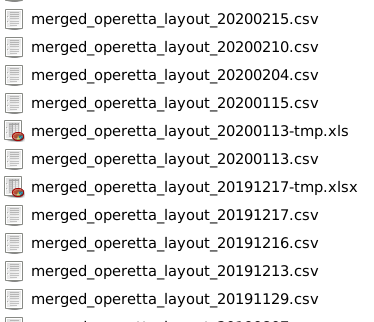
\includegraphics[height=160pt]{pictures/Screenshot_2020-02-25_17-47-03-ugly_folder-zoom_in.png}

\end{frame}

\begin{frame}

\begin{itemize}
	\item the state of the art solution
	\begin{itemize}
		\item  have one file in the working directory
		\item store the old versions 'hidden' in a \textbf{repository}
	\end{itemize}
	\pause
	\item What is a \textbf{repository}?
	\begin{itemize}
		\item  a simple subfolder 
		\item The folder name is '.git'.
		\item It is a hidden forlder
		\item You have to start git to see the content
	\end{itemize}
\end{itemize}

\end{frame}

\begin{frame}
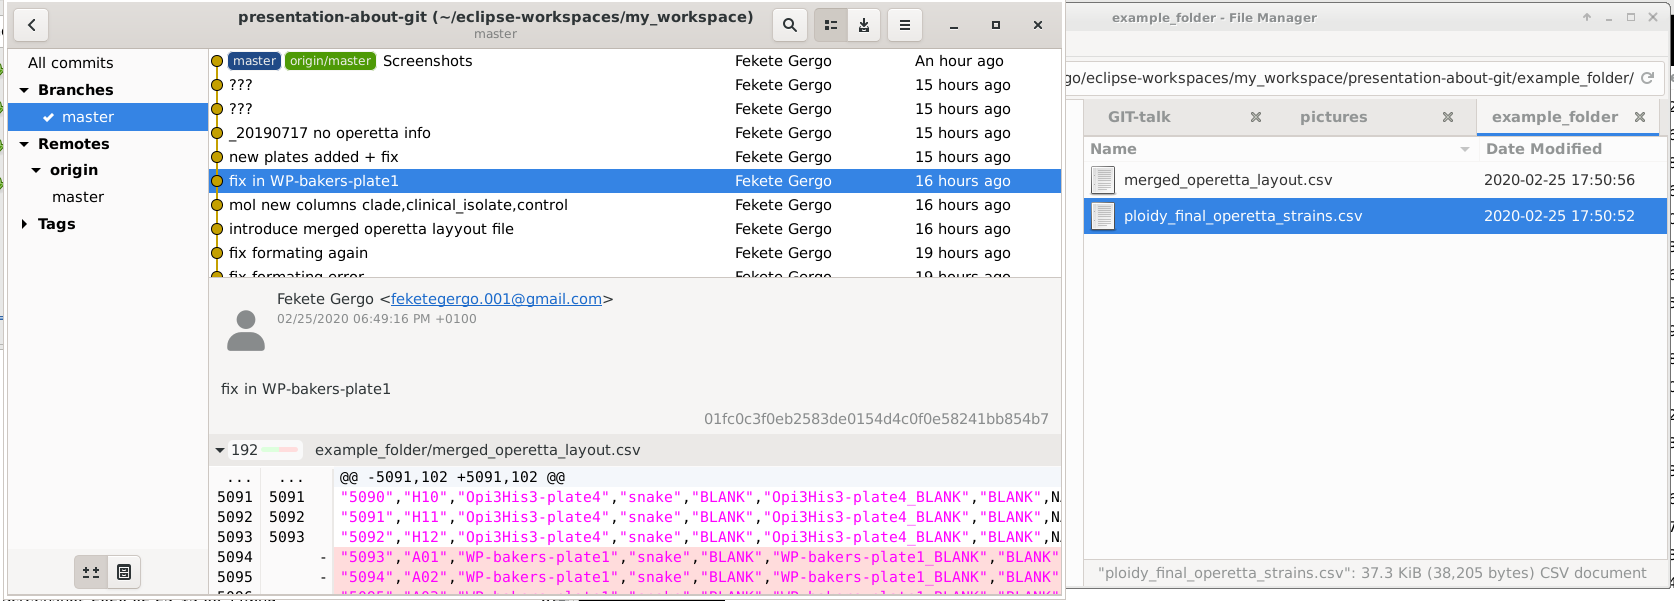
\includegraphics[height=120pt]{pictures/Screenshot_2020-02-26_10-21-26-folder_in_git.png}

\begin{itemize}
	\item normally you see only the 2 important files 
	\item If you need the old versions you can turn on the repository browser.
	\pause
	\item Each ball represents a prevoius version
	\item the term of the 'balls' is commit/revision/version
	\pause
	\item You can delete files from the working directory.The repo keeps it.
\end{itemize}
\end{frame}

\begin{frame}
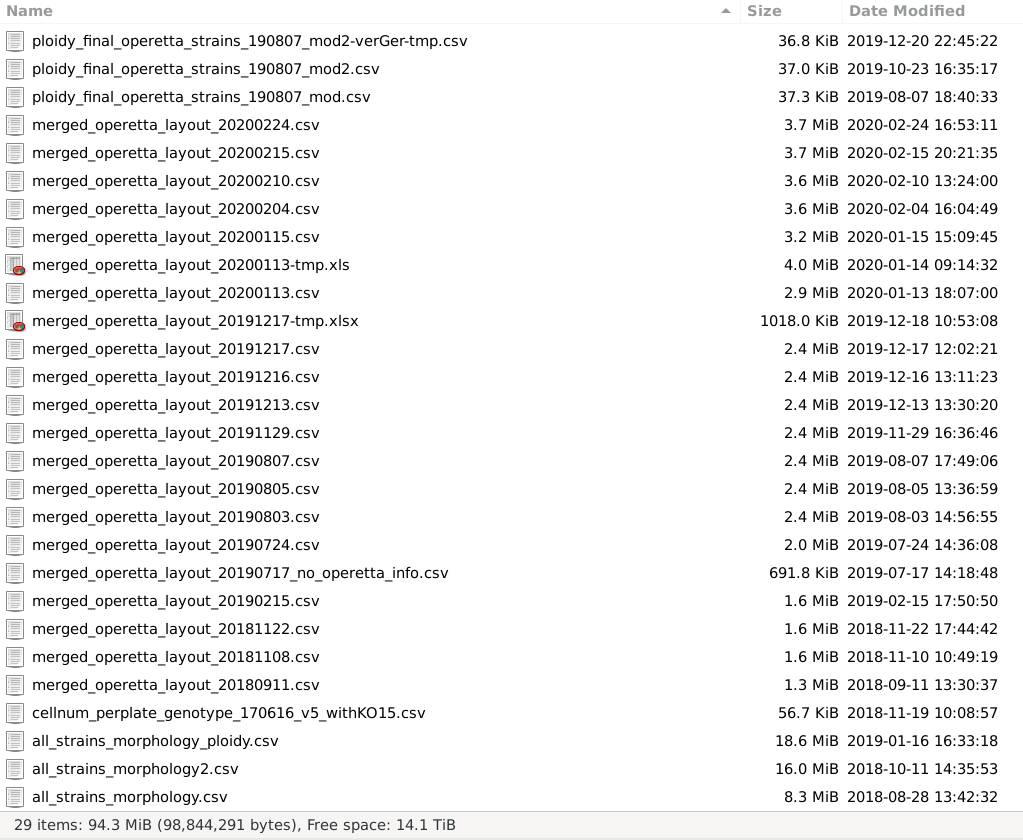
\includegraphics[height=120pt]{pictures/Screenshot_2020-02-25_17-47-03-ugly_folder.png}

\begin{itemize}
		\item working with messy forlders is slower and comfusing
		\item it causes errors
		\item It is waste of time and money.
	\end{itemize}

\end{frame}


\begin{frame}

  Back to the top
  
	\begin{block}{GIT}
		GIT is a  tool to save folders , and handle versions
	\end{block}
  
	\begin{itemize}
  		\item now we know what are versions
		\item Let's see why to save forlders instead of files
	\end{itemize}

\end{frame}


\begin{frame}
\frametitle<presentation>{Why to save forlders?}

Belive me! It is a result of 35 years of evoluton and desig. 

\end{frame}

\begin{frame}
\frametitle<presentation>{Why to save forlders?}

Imagine a project where are 
\begin{itemize}
  		\item experimental layout file
		\item result files form a microscoope
\end{itemize}
\pause
They belong together. It is nice to connect them.
\pause
\begin{itemize}
  		\item actually it does not save full forlder. You can select some files to save together.
		\item The principal concept is 'comit together what belongs together'
\end{itemize}


\end{frame}




\begin{frame}
\frametitle<presentation>{Back to the top again}
  
  
	\begin{block}{GIT}
		GIT is a  tool to save folders , and handle versions
	\end{block}
  
	\begin{itemize}
  		\item now we know what are versions
		\item we undarstand that commit many files together is clever
		\pause
		\item What is the GIT tool?
	\end{itemize}

\end{frame}

\begin{frame}
\frametitle<presentation>{What is the GIT tool?}

	\begin{itemize}
  		\item actually git is not one tool: it is a protocol/standard
		\item There arae a lot of git program you can install.
	\end{itemize}
\pause
	\begin{itemize}
  		\item Linux and Mac have preinstalled git
		\item Rstudio contains a git client
		\item every IDE contains a git client (C , JAVA, pyton editors \ldots)
	\end{itemize}
\pause
	\begin{itemize}
  		\item gitg  (grafikal UI - linux, windows, mac)
		\item git SMC (Window git client)
		\item Git Bash (Window git terminal)
		\item every IDE contains a git client (C , JAVA, pyton editors \ldots)
	\end{itemize}


\end{frame}





\begin{frame}
\frametitle<presentation>{Let's see how to use it}
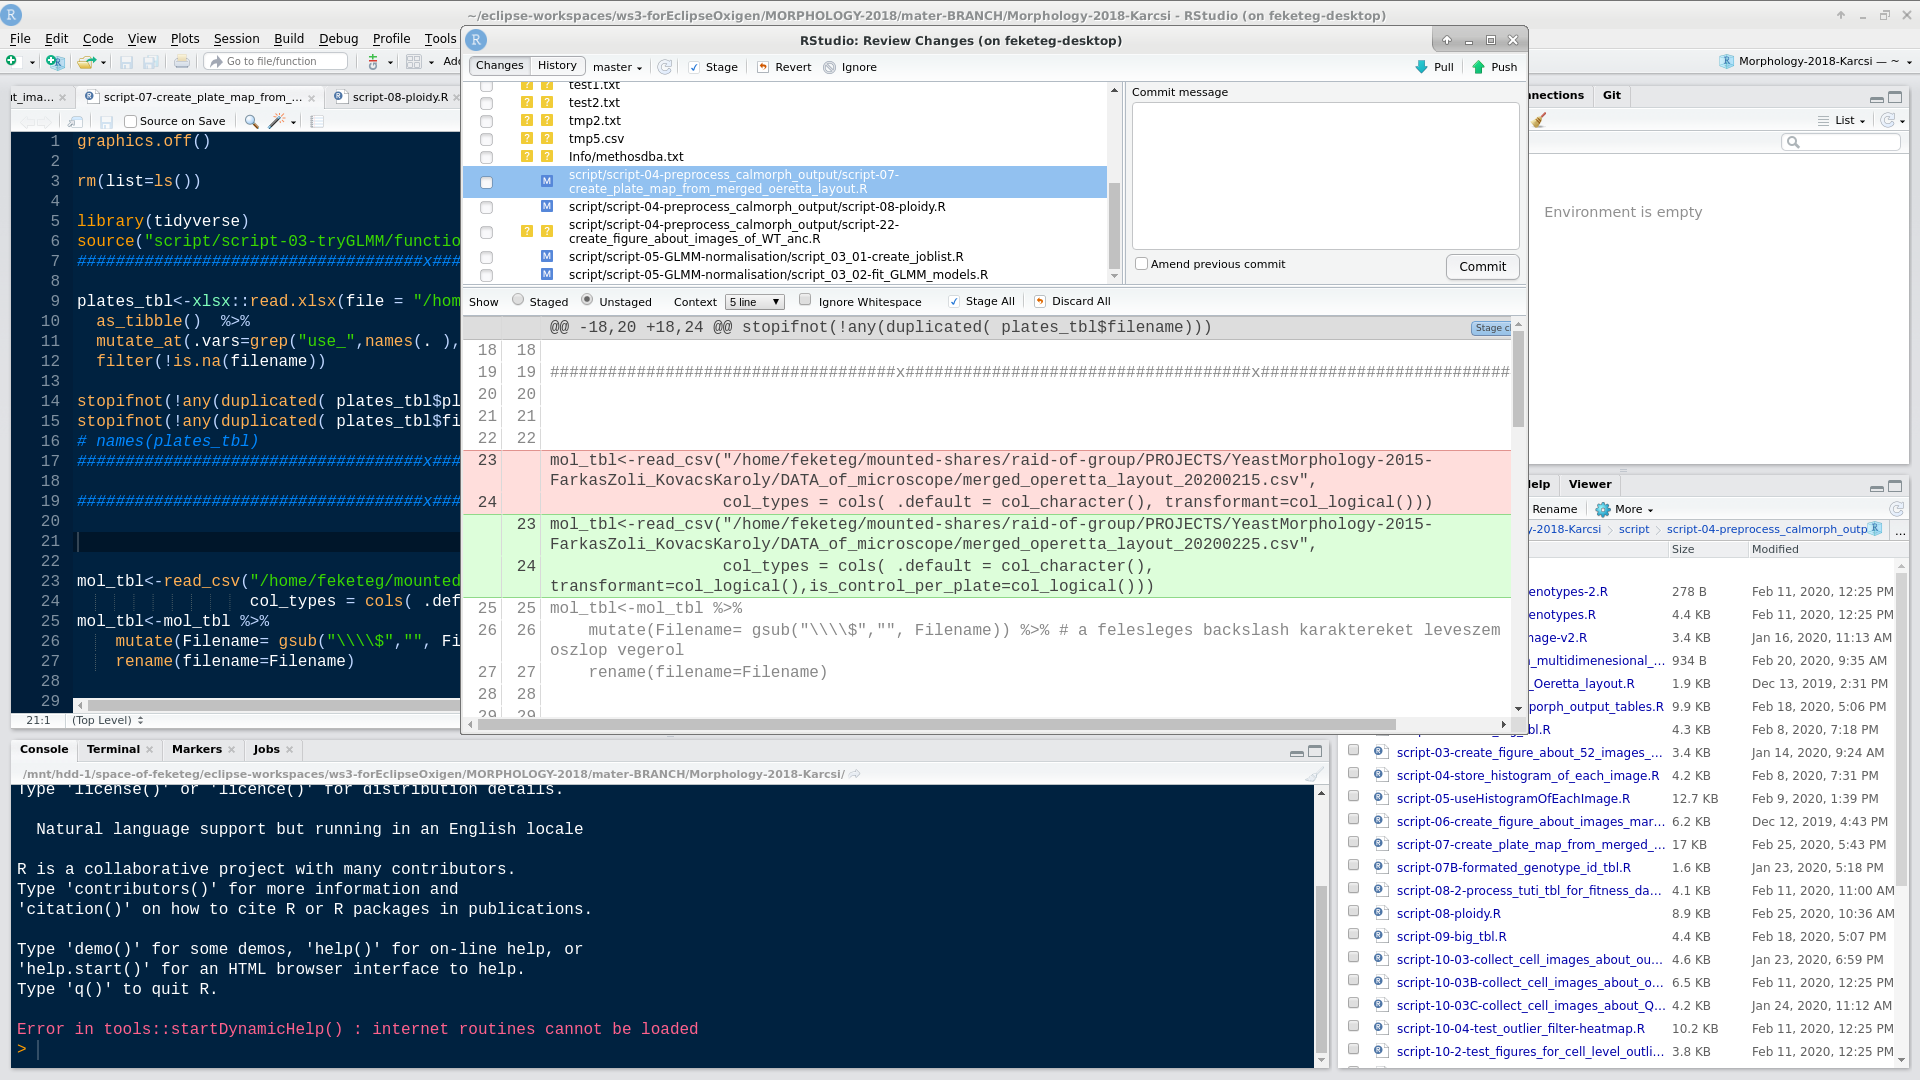
\includegraphics[height=180pt]{pictures/Screenshot_2020-02-26_08-48-52-rstudio-commit-window.png}

\end{frame}

\begin{frame}
\frametitle<presentation>{Let's see how to use it}
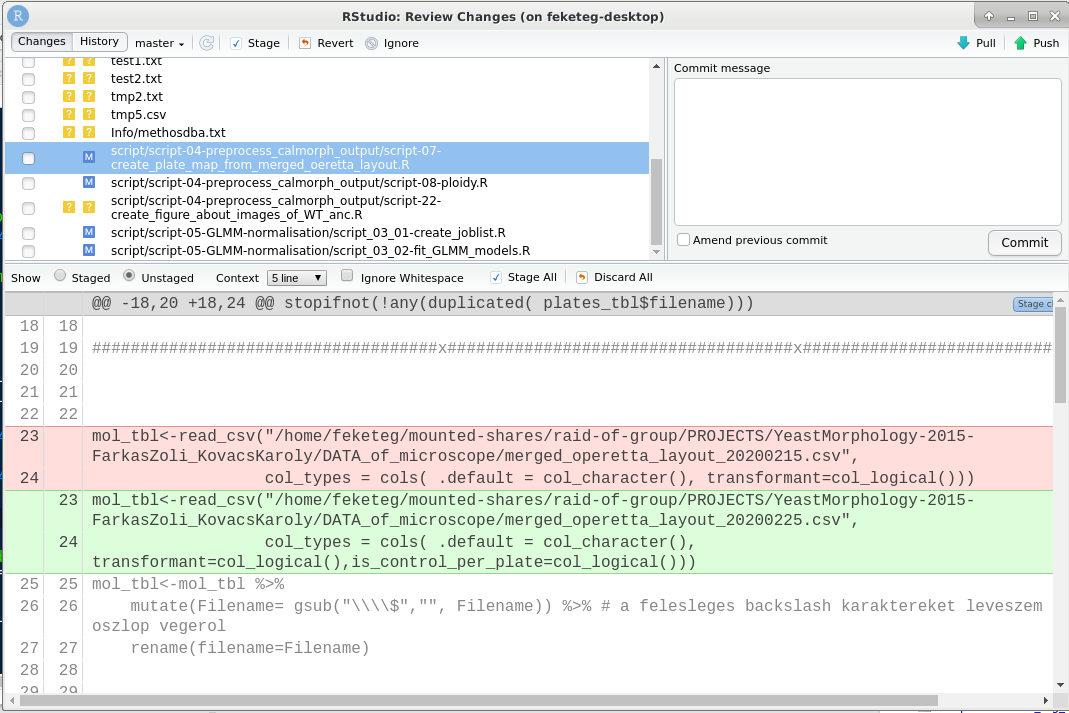
\includegraphics[height=180pt]{pictures/Screenshot_2020-02-26_08-48-52-rstudio-commit-window-zoom_in.png}

\end{frame}

\begin{frame}
\frametitle<presentation>{Let's see how to use it}
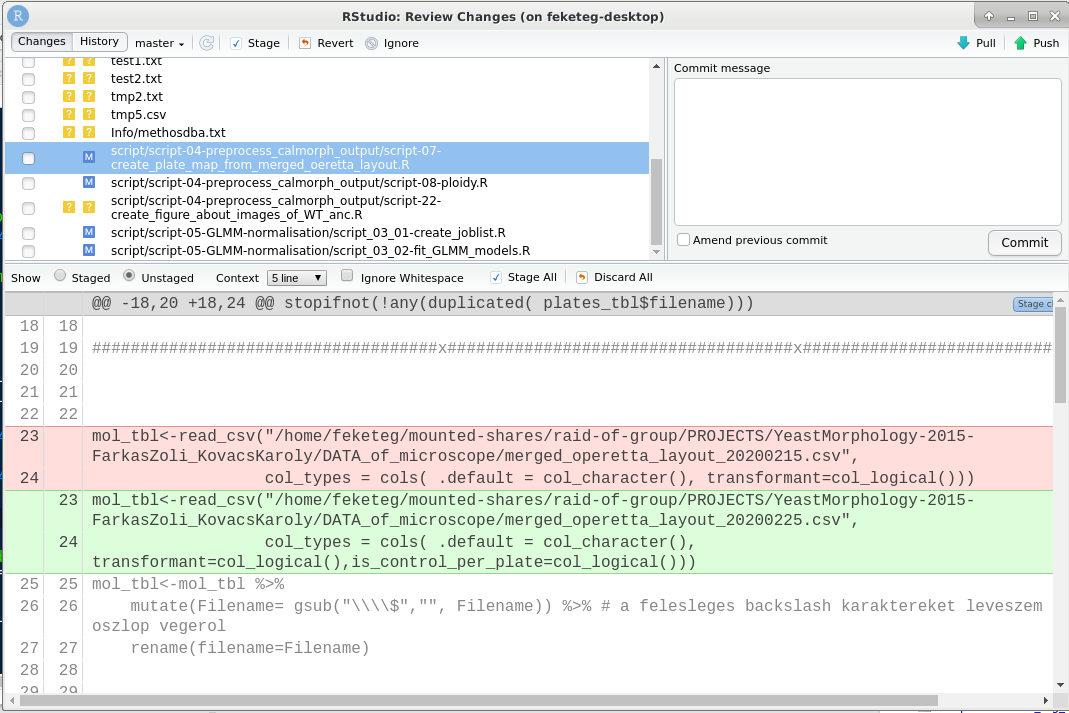
\includegraphics[height=100pt]{pictures/Screenshot_2020-02-26_08-48-52-rstudio-commit-window-zoom_in.png}

\begin{itemize}
  		\item select files to the stage
  		\item unfullowed/followed files
		\item diff-s 
		\item commit msg + button
		\item push/pull button
	\end{itemize}
\end{frame}

\begin{frame}
\frametitle<presentation>{Terminology}

\begin{itemize}
  		\item commit = save it (to the local repository)
  		\item stage = files selected for save
		\item push = upload to the server 
		\item pull = download from the server
	\end{itemize}
\end{frame}


\begin{frame}
\frametitle<presentation>{Let's see how to use it - History}
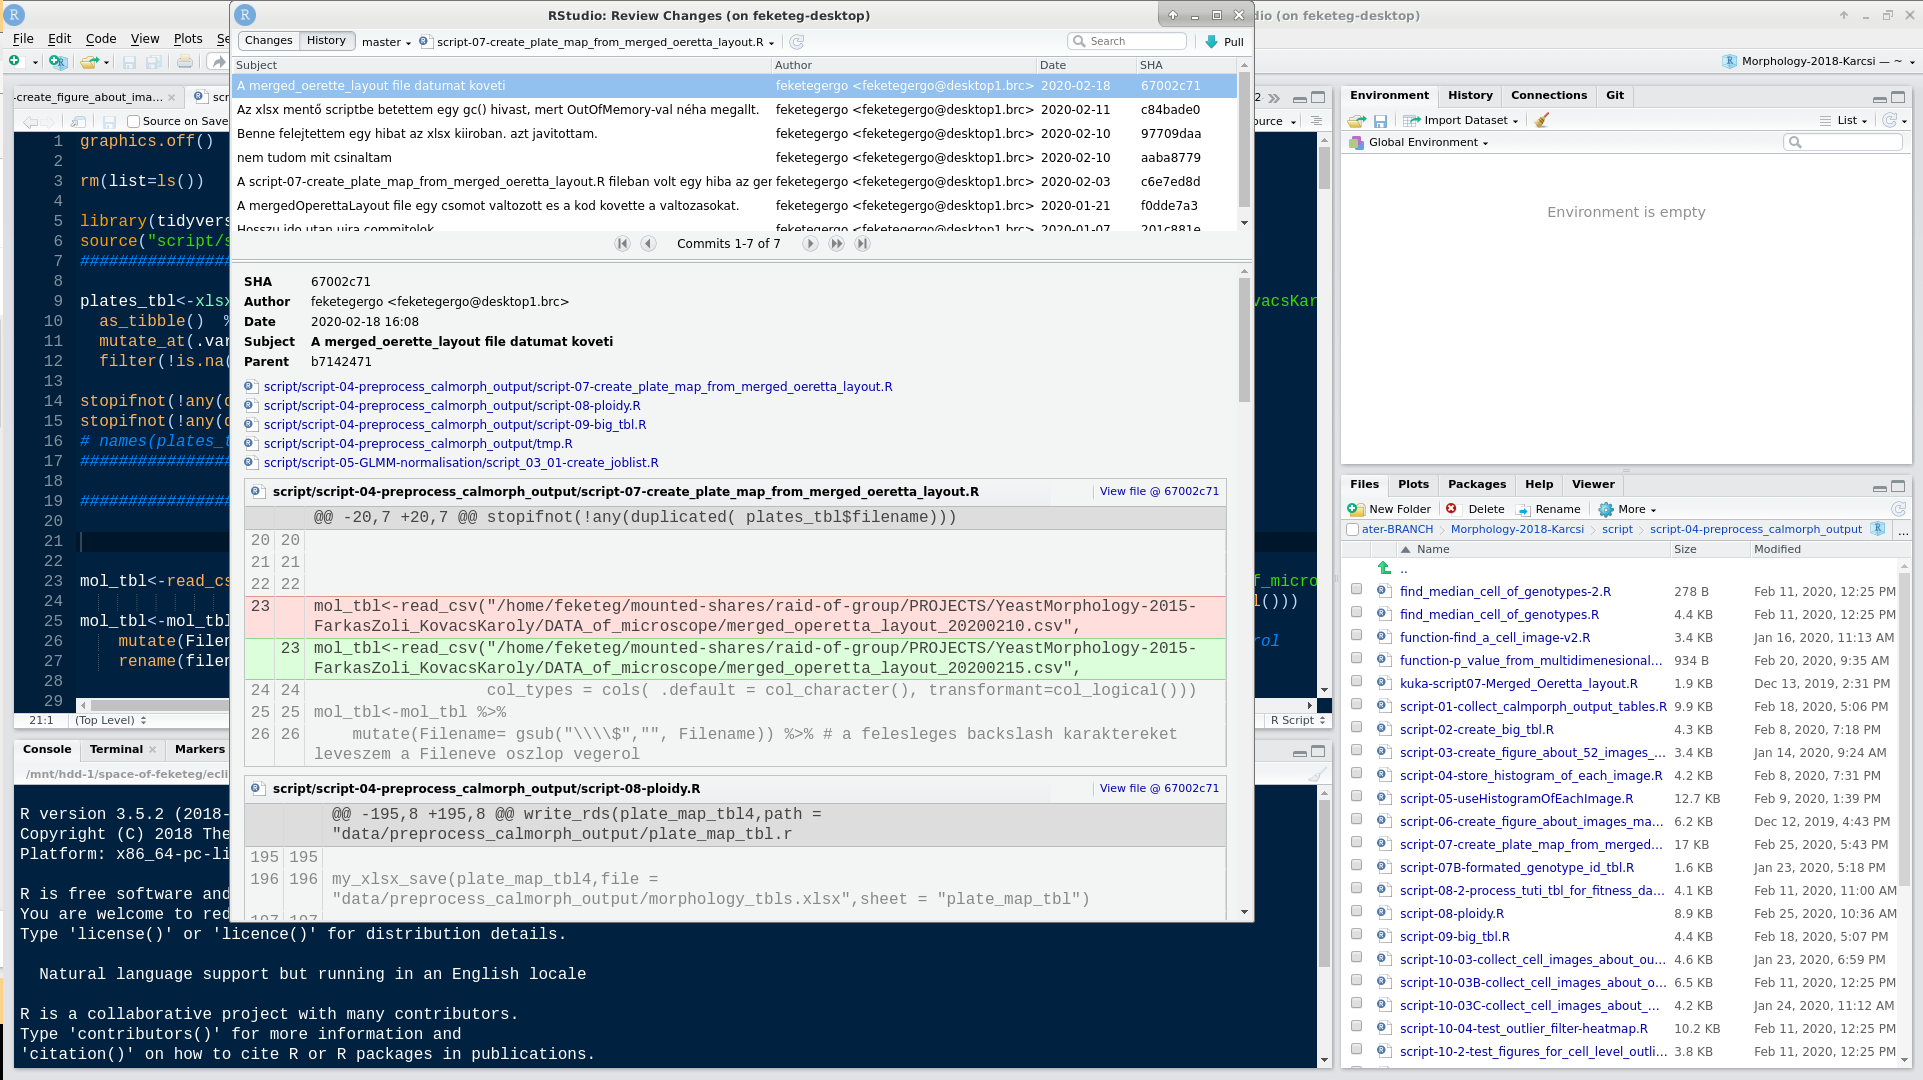
\includegraphics[height=180pt]{pictures/Screenshot_2020-02-26_08-38-28-Rstudio-Git-history.png}
\end{frame}

\begin{frame}
\frametitle<presentation>{Let's see how to use it- History}
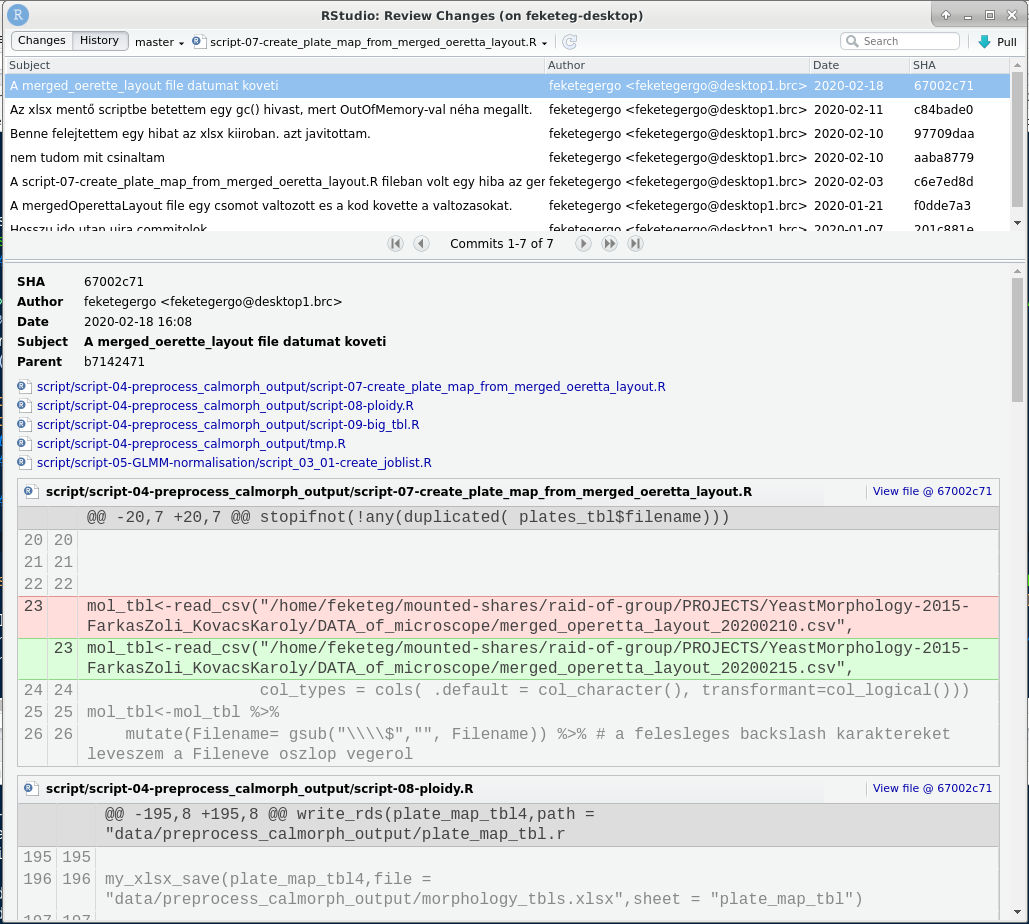
\includegraphics[height=180pt]{pictures/Screenshot_2020-02-26_08-38-28-Rstudio-Git-history-zoom_in.png}
\end{frame}


\begin{frame}
\frametitle<presentation>{Let's see how to use it- History}
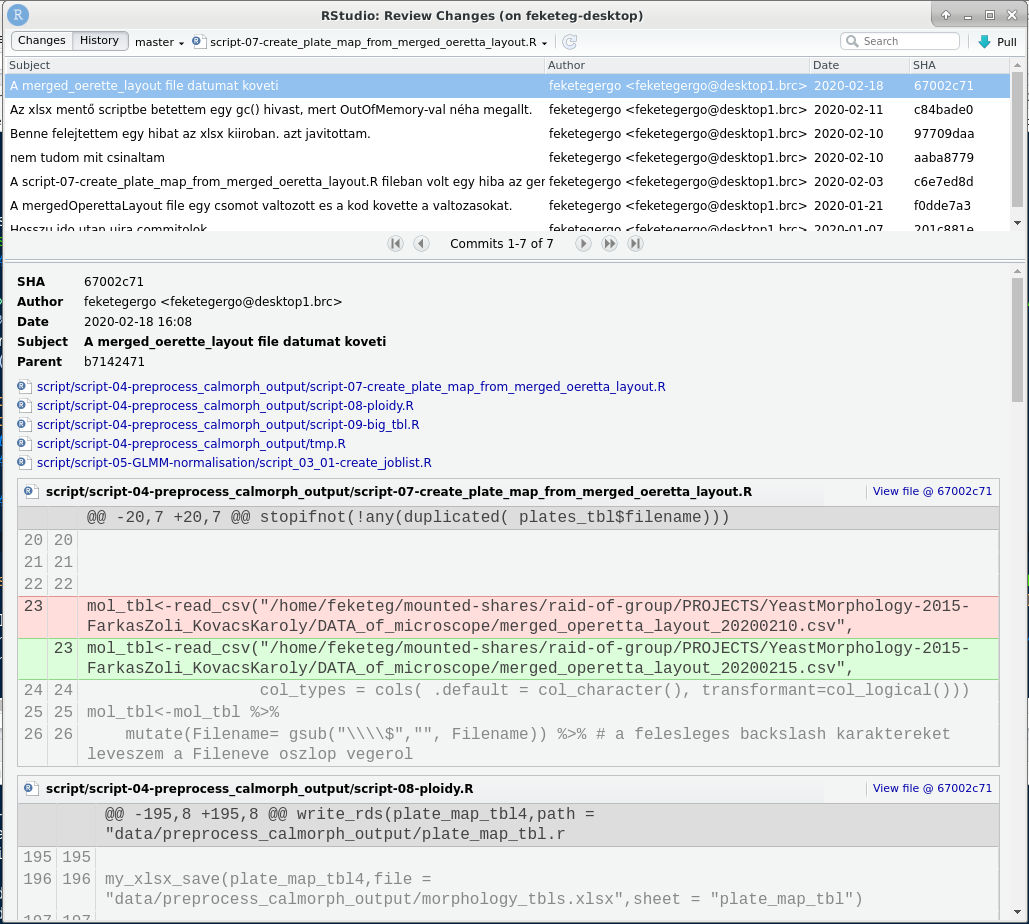
\includegraphics[height=80pt]{pictures/Screenshot_2020-02-26_08-38-28-Rstudio-Git-history-zoom_in.png}

\begin{itemize}
  		\item each row is a commit with
	  		\begin{itemize}
	  		\item date
	  		\item author
			\item comment 
			\item commit ID
			\end{itemize}
  		\item list of files modified in the selected commit 
  		\item diffs : for each file it shows what is modified
	\end{itemize}
\end{frame}


\begin{frame}
\frametitle<presentation>{Principles}

\begin{itemize}
  		\item If you want to roll back 
	  		\begin{itemize}
	  		\item You have to commit first
	  		\item git will replace the actual files with the old ones
			\item You can not rollback only one file. 
			\end{itemize}
  		\item You can go back to an old version and then return to the latest version 
  		\item If you want to go somewhere you have to tell the ID of the version 
  		\item the last commit called \textbf{HEAD}
  		\item the 'go to' command is \textbf{checkout}
	\end{itemize}

\begin{block}{Example}
		git checkout 67002c71
	\end{block}
  
  \begin{block}{}
		git checkout HEAD
	\end{block}
  
\end{frame}

\begin{frame}
\frametitle<presentation>{Principles}

\begin{block}{bad news}
		sometimes you need to type commands
\end{block}
\end{frame}

   
\begin{frame}
\frametitle<presentation>{GitHub}



\begin{block}{GitHub}
GitHub is a webserver where you can save 
\end{block}

\begin{itemize}
\item GIT saves things to the local repository on your machine
\item GIT can upload everything to a remote git-server
\item GitHub is one of the git servers
\end{itemize}
 
\end{frame}


\section{GitHub}

\begin{frame}

\begin{block}{GitHub}
GitHub is a webserver where you can save 
\end{block}

\begin{itemize}
\item GIT saves things to the local repository on your machine
	\begin{itemize}
		\item local repository needs to exist
	\end{itemize}
\pause
\item GIT can upload everything to a remote git-server
	\begin{itemize}
		\item does not upload the actual files.
		\item uploads the repository: all versions
	\end{itemize}
\pause
	
\item GitHub is one of the git servers
	\begin{itemize}
		\item Bitbucket
		\item Gitlab
		\item We can hawe our own git server 
	\end{itemize}
\end{itemize}
 
\end{frame}




\begin{frame}


\begin{itemize}
\item basic git servers just stores the repository
\item GitHub provides additional Web interface
\end{itemize}


\begin{figure}[ht]
\centering
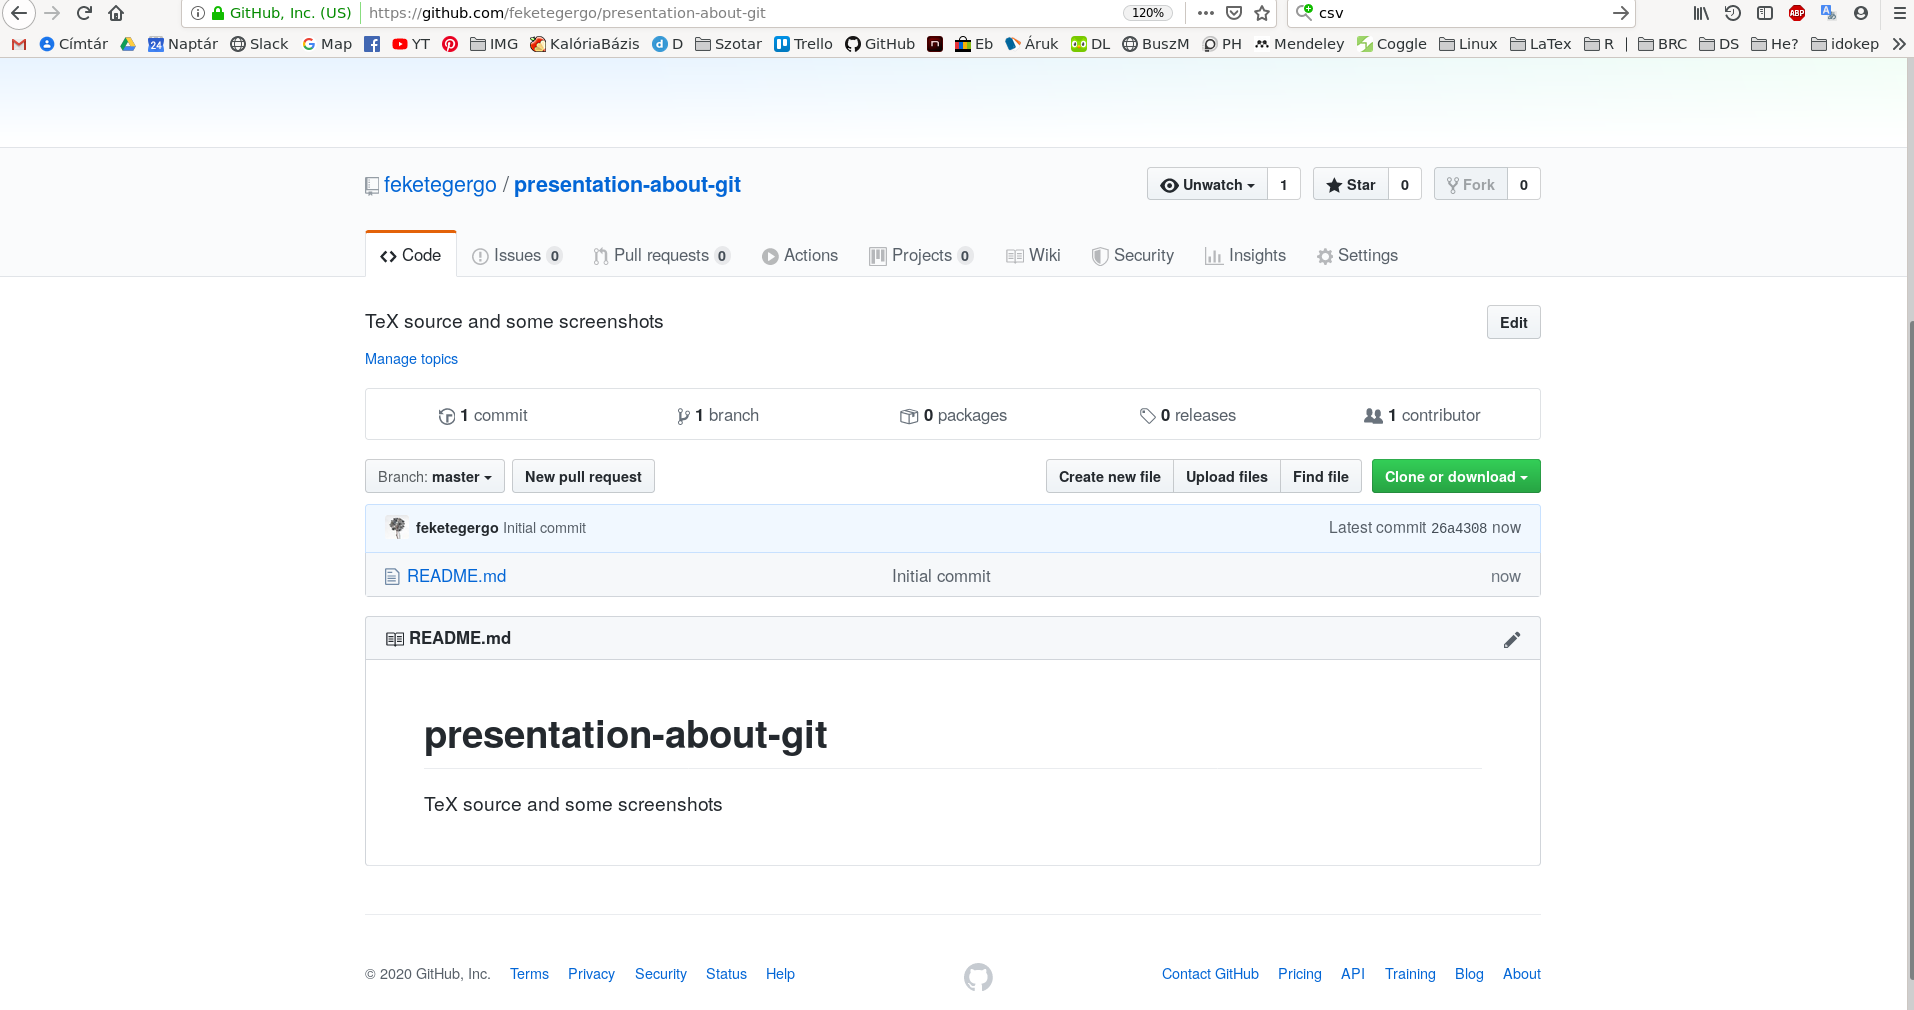
\includegraphics[height=120pt]{pictures/Screenshot_2020-02-25_14-38-35.png}
\end{figure}

 
\end{frame}



\begin{frame}
\frametitle<presentation>{Start a GitHub Project}



\begin{itemize}
\item go to github.com , register a user
\item create a new project. Tick the 'initialised' checkbox.
\item copy paste the url of the project  
\item start a terminal, go to the parent folder.
\item use 'git clone <\textit{url}>' command 
\end{itemize}

\pause

\begin{itemize}
\item now you have an initialised local repository in the folder
\item the \textbf{clone} command automaticly connected it to the GitHub repo.

\item you can commit files.  
\item if you press the 'push' button or give the 'git push' command, then everything will be uploaded.
\item If another user modified the files on the server the  'git pull' command download it 
\end{itemize}


\end{frame}



\begin{frame}
\frametitle<presentation>{Tricky things start here}



\begin{itemize}
\item If you try to upload a file, what is modified by another user\ldots.
\pause
\item It is called 'conflict'
\item The operetion 'merge' can fix the problem  
\item normaly git merge it automaticly
\item pull first then push 
\end{itemize}


 
\end{frame}





\begin{frame}
\begin{figure}[ht]
\centering
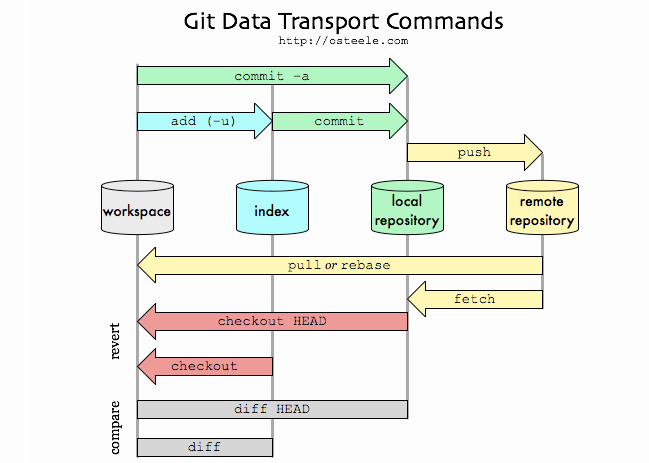
\includegraphics[height=150pt]{pictures/git.jpg}
\end{figure}
\end{frame}






\begin{frame}
\begin{figure}[ht]
\centering
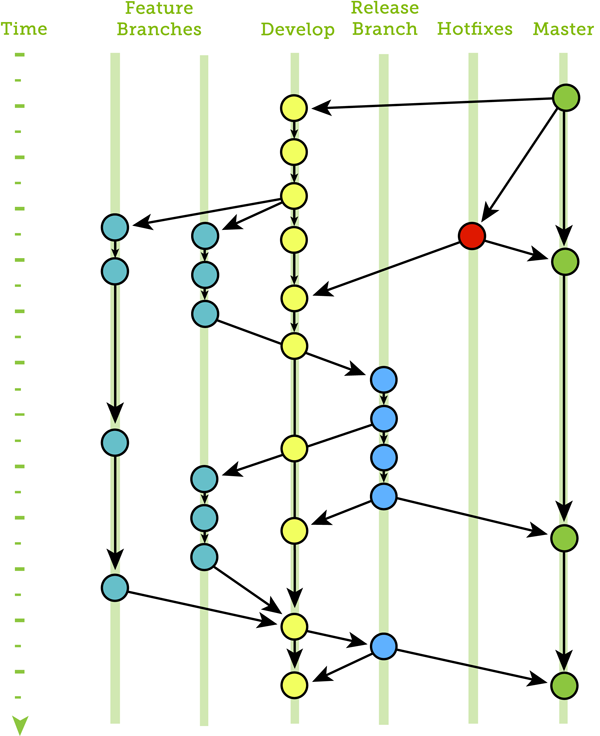
\includegraphics[height=150pt]{pictures/branches.jpg}
\end{figure}
\end{frame}




\end{document}


